\documentclass{article}
\usepackage{pgfplots}
\pgfplotsset{compat=1.17}

\begin{document}

\begin{figure}[h]
    \centering
    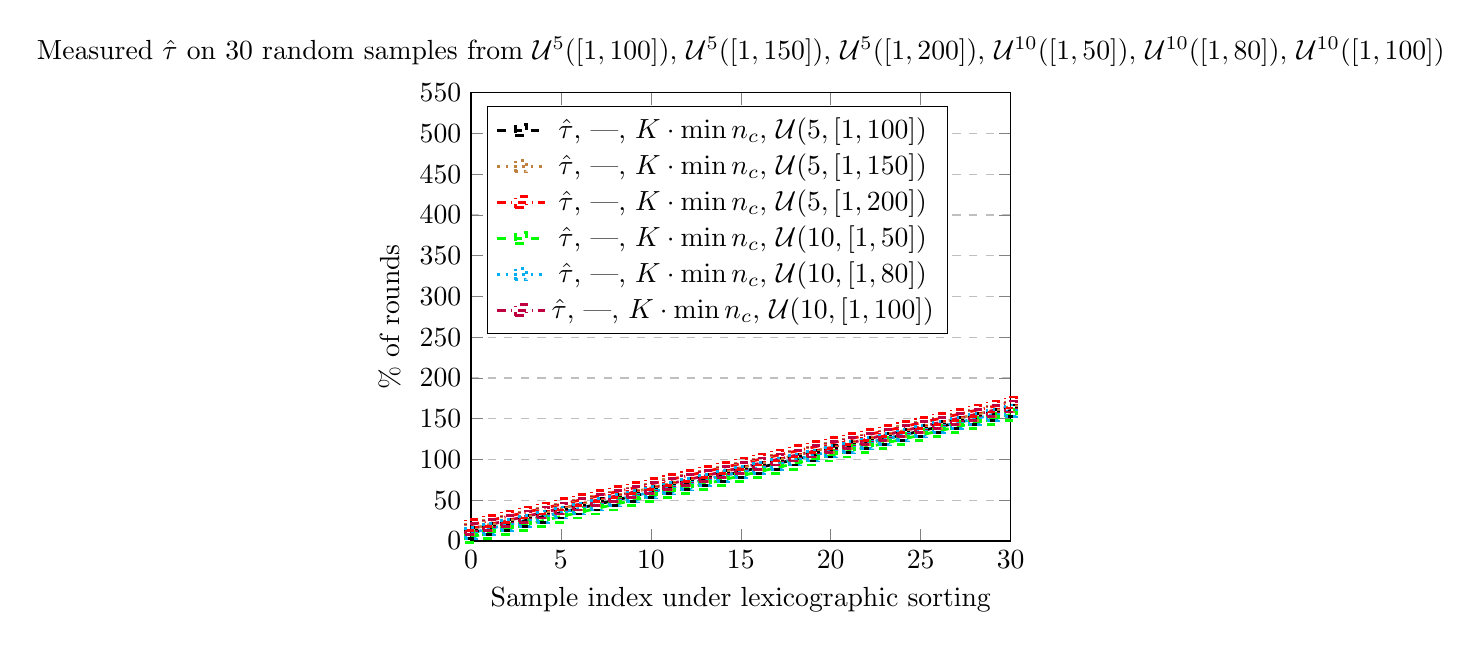
\begin{tikzpicture}
        \begin{axis}[
            title={Measured $\hat{\tau}$ on 30 random samples from $\mathcal{U}^5([1,100])$, $\mathcal{U}^5([1,150])$, $\mathcal{U}^5([1,200])$, $\mathcal{U}^{10}([1,50])$, $\mathcal{U}^{10}([1,80])$, $\mathcal{U}^{10}([1,100])$},
            xlabel={Sample index under lexicographic sorting},
            ylabel={$\%$ of rounds},
            xmin=0, xmax=30,
            ymin=0, ymax=550,
            xtick={0,5,...,30},
            ytick={0,50,...,550},
            legend pos=north west,
            ymajorgrids=true,
            grid style=dashed,
        ]
            \addplot[
                color=black,
                mark=square,
                dashed,
                line width=1pt,
                ]
                coordinates {
                    (0,10)(1,15)(2,20)(3,25)(4,30)(5,35)(6,40)(7,45)(8,50)(9,55)(10,60)(11,65)(12,70)(13,75)(14,80)(15,85)(16,90)(17,95)(18,100)(19,105)(20,110)(21,115)(22,120)(23,125)(24,130)(25,135)(26,140)(27,145)(28,150)(29,155)(30,160)
                };
            \addlegendentry{$\hat{\tau}$, ---, $K \cdot \min{n_c}$, $\mathcal{U}(5,[1,100])$}
            
            \addplot[
                color=brown,
                mark=square,
                dotted,
                line width=1pt,
                ]
                coordinates {
                    (0,15)(1,20)(2,25)(3,30)(4,35)(5,40)(6,45)(7,50)(8,55)(9,60)(10,65)(11,70)(12,75)(13,80)(14,85)(15,90)(16,95)(17,100)(18,105)(19,110)(20,115)(21,120)(22,125)(23,130)(24,135)(25,140)(26,145)(27,150)(28,155)(29,160)(30,165)
                };
            \addlegendentry{$\hat{\tau}$, ---, $K \cdot \min{n_c}$, $\mathcal{U}(5,[1,150])$}
            
            \addplot[
                color=red,
                mark=square,
                dashdotted,
                line width=1pt,
                ]
                coordinates {
                    (0,20)(1,25)(2,30)(3,35)(4,40)(5,45)(6,50)(7,55)(8,60)(9,65)(10,70)(11,75)(12,80)(13,85)(14,90)(15,95)(16,100)(17,105)(18,110)(19,115)(20,120)(21,125)(22,130)(23,135)(24,140)(25,145)(26,150)(27,155)(28,160)(29,165)(30,170)
                };
            \addlegendentry{$\hat{\tau}$, ---, $K \cdot \min{n_c}$, $\mathcal{U}(5,[1,200])$}
            
            \addplot[
                color=green,
                mark=square,
                dashed,
                line width=1pt,
                ]
                coordinates {
                    (0,5)(1,10)(2,15)(3,20)(4,25)(5,30)(6,35)(7,40)(8,45)(9,50)(10,55)(11,60)(12,65)(13,70)(14,75)(15,80)(16,85)(17,90)(18,95)(19,100)(20,105)(21,110)(22,115)(23,120)(24,125)(25,130)(26,135)(27,140)(28,145)(29,150)(30,155)
                };
            \addlegendentry{$\hat{\tau}$, ---, $K \cdot \min{n_c}$, $\mathcal{U}(10,[1,50])$}
            
            \addplot[
                color=cyan,
                mark=square,
                dotted,
                line width=1pt,
                ]
                coordinates {
                    (0,10)(1,15)(2,20)(3,25)(4,30)(5,35)(6,40)(7,45)(8,50)(9,55)(10,60)(11,65)(12,70)(13,75)(14,80)(15,85)(16,90)(17,95)(18,100)(19,105)(20,110)(21,115)(22,120)(23,125)(24,130)(25,135)(26,140)(27,145)(28,150)(29,155)(30,160)
                };
            \addlegendentry{$\hat{\tau}$, ---, $K \cdot \min{n_c}$, $\mathcal{U}(10,[1,80])$}
            
            \addplot[
                color=purple,
                mark=square,
                dashdotted,
                line width=1pt,
                ]
                coordinates {
                    (0,15)(1,20)(2,25)(3,30)(4,35)(5,40)(6,45)(7,50)(8,55)(9,60)(10,65)(11,70)(12,75)(13,80)(14,85)(15,90)(16,95)(17,100)(18,105)(19,110)(20,115)(21,120)(22,125)(23,130)(24,135)(25,140)(26,145)(27,150)(28,155)(29,160)(30,165)
                };
            \addlegendentry{$\hat{\tau}$, ---, $K \cdot \min{n_c}$, $\mathcal{U}(10,[1,100])$}
        \end{axis}
    \end{tikzpicture}
    \caption{Measured $\hat{\tau}$ on 30 random samples from $\mathcal{U}^5([1,100])$, $\mathcal{U}^5([1,150])$, $\mathcal{U}^5([1,200])$, $\mathcal{U}^{10}([1,50])$, $\mathcal{U}^{10}([1,80])$, $\mathcal{U}^{10}([1,100])$.}
    \label{fig:measured_tau}
\end{figure}

\end{document}